

%%%%%%%%%%%%%%%%%%%%%%%%%%%%%%%%%%%%%%%%%%%%%%
\section{Muon Tagger}
\label{sec:beam:muontagger}

%%%%%%%%%%%%%%%%%%%%%%%%%%
\subsection{Overview}

The ProtoDUNE-SP muon tagger, called the Cosmic Ray Tagger (CRT), enables tagging and reconstruction of muons crossing the TPC volume. The ProtoDUNE-SP CRT is an assembly of modules based on the muon module and readout electronics designs used for the Double Chooz large-area muon-tagging system, called the Outer Veto.  
%
The CRT will provide a sample of tracked comic-ray muons (and beam halo muons), with known $t0$'s, to map out the effects of space charge, which are expected to be large. It will also aid in measuring the electron lifetime in the TPC.

Whereas the Double Chooz Outer Veto modules are installed above the detector, the ProtoDUNE-SP CRT modules will be installed on the upstream and downstream sides of the detector.
These modules are highly segmented, and are layered in $x$ and $y$ so as to provide 2D coordinates over much of the detector's cross sectional area.  
The modules have been fully tested following construction at the University of Chicago, and are currently stored in Strasbourg. The PMTs and front-end electronics, originally produced at Columbia University, are stored at Virginia Tech.
\fixme{is the location info necessary?  most components don't provide this info}

%The ProtoDUNE CRT will make use of muon modules and readout electronics constructed for the Double Chooz Outer Veto, a large-area muon tagging system installed above the Double Chooz detector. As described below, these modules will be layered to provide two-dimensional coordinates over much of the upstream and downstream faces of ProtoDUNE. These highly segmented modules, all of which have been fully tested following construction at the University of Chicago, are currently stored in Strasbourg. All of the PMTs and front-end electronics, originally produced at Columbia University, are stored at Virginia Tech.


%%%%%%%%%%%%%%%%%%%%%%%%%%
\subsection{CRT module design and readout}

%The CRT is an assembly of modules, 
Each CRT module contains 64 5-cm $\times$ 1-cm $\times$ 320-cm scintillator strips in two 32-strip layers. The layers are 2.5\,cm apart. 
\fixme{layers or wire pitch?}
Each scintillator strip has a 1.5-mm diameter wavelength-shifting fiber inserted into a hole created during the extrusion process.  The resulting modules are 1.625-m wide and 3.6-m long (see Figures~\ref{fig:one-crt-module} and~\ref{fig:crt-module-photo}). 
\fixme{the photo is not instructive - you can't see wires or layers}
The 64 wavelength-shifting fibers on one end (right-hand side of  Figure~\ref{fig:one-crt-module})
are coupled to a Hamamatsu M64 multi-anode photomultiplier tube (PMT); the other fiber ends are mirrored. 
\fixme{I don't know what that means}
Each M64 is connected to a custom front-end board with a MAROC2 ASIC and an FPGA. 
\fixme{inset in fig 2}
The MAROC2 allows adjustment of the electronic gain of each of the 64 channels; this is needed to correct for the factor-of-two pixel-to-pixel gain variation in the M64.  Signals that exceed a common threshold are sent to a multiplexed 12-bit ADC, providing pulse height information for hit strips. The readout of each module is self-triggered. Each module requires a 62.5-MHz clock and a sync pulse. The sync pulse is a NIM signal that should have 
\fixme{has? or is expected to have? ``should have'' is not clear enough}
a frequency between 0.5 and 0.05\,Hz. The sync signal is used to reset the internal counter of each module. 
A muon-like signal in a module, i.e., a signal that creates overlapping hits in the two layers, produces a single NIM trigger output.
%Each module produces a single NIM trigger output indicating the presence of a muon-like signal (i.e., overlapping hits in the two module layers).

\begin{cdrfigure}[Drawing of Cosmic Ray Tagger (CRT) module]{one-crt-module}{Drawing of one 64-strip CRT module (one 32-strip layer shown).  Each module contains two layers of 32 5-cm $\times$ 1-cm $\times$ 320-cm strips with wavelength-shifting fibers.  The 64 fibers for each module are coupled to a Hamamatsu M64.}
  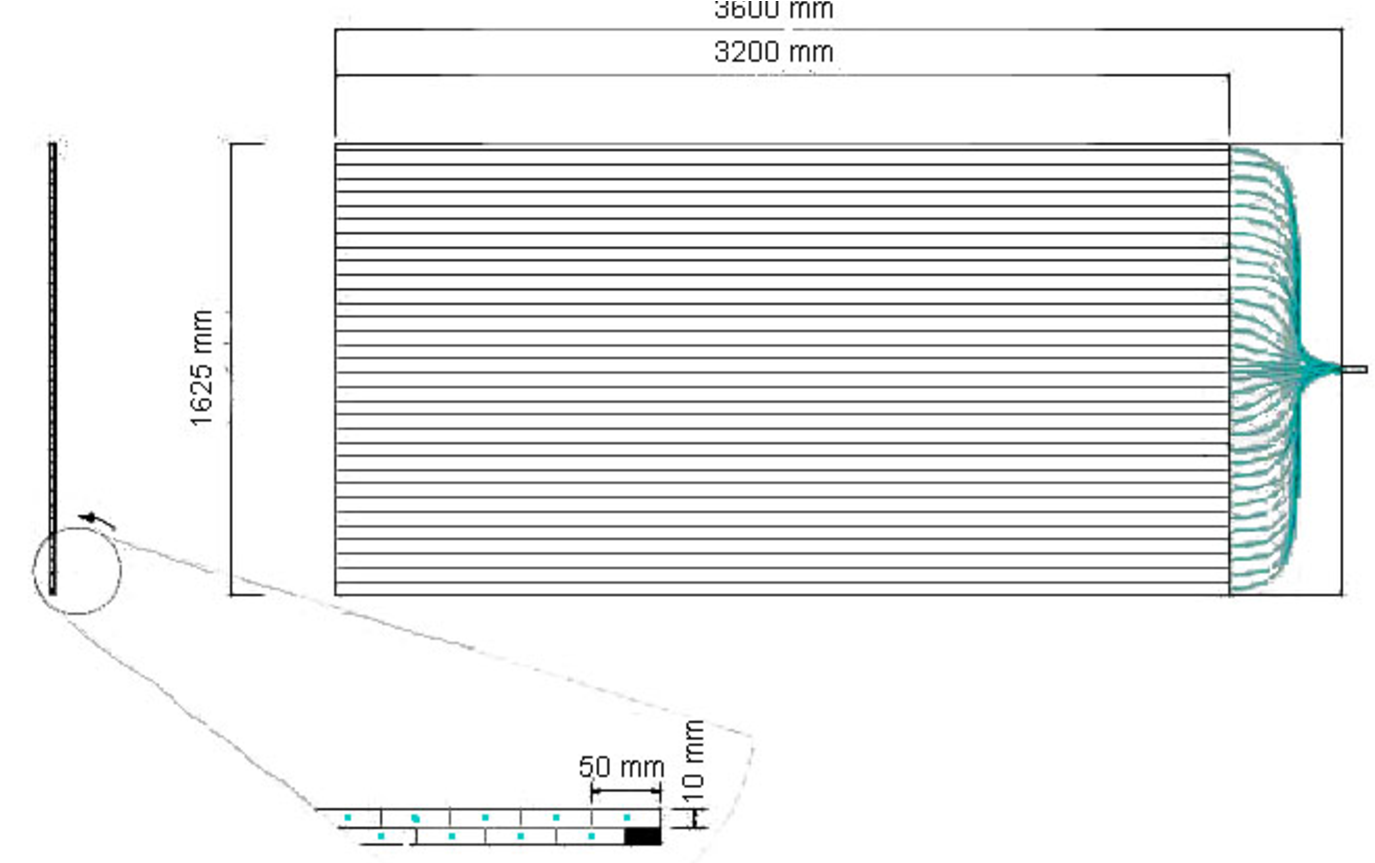
\includegraphics[width=0.7\textwidth]{one-crt-module}
\end{cdrfigure}

\begin{cdrfigure}[Photo of CRT module]{crt-module-photo}{Photo of CRT module. The inset shows the front-end board attached to the PMT and module. The two large chips are the MAROC2 and an Altera FPGA.}
  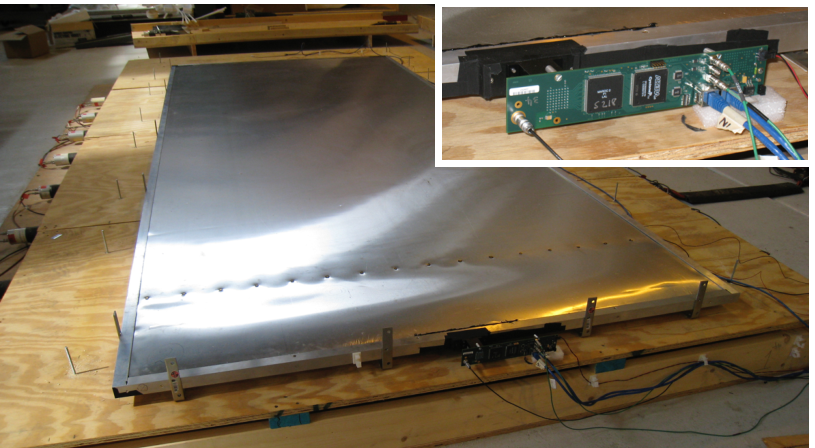
\includegraphics[width=0.8\textwidth]{crt-module-photo}
\end{cdrfigure}

%%%%%%%%%%%%%%%%%%%%%%%%%%
\subsection{Layout of CRT modules}

The ProtoDUNE-SP CRT is based on units of four modules, two with strips oriented in the $x$ direction and two with strips oriented in the $y$ direction (see Figure~\ref{fig:crt-layout}). These four-module units result in a 3.2-m $\times$ 3.2-m area with 2D readout with 2.5-cm pitch.
\fixme{put pitch in prev section?}
\fixme{wait, I thought in ONE module there is an x and a y layer. This sounds like each module is either x or y, then you put modules together in different orientations. which is right?}

The Double Chooz modules were designed to be installed horizontally, but the ProtoDUNE-SP modules are installed vertically. Tests are currently underway to evaluate two schemes for holding the modules. Following these small-scale tests, a full prototype structure with a real module will be constructed and tested in Chicago.

\begin{cdrfigure}[Layout of four-module CRT unit and photo of similar one]{crt-layout}{(left) Layout of four-module unit, providing 2D readout over a 3.2-m $\times$ 3.2-m region. The red regions represent the inactive parts of the modules, where fibers are routed to the M64s. (right) Photo of similar four-module layout at Double Chooz.}
  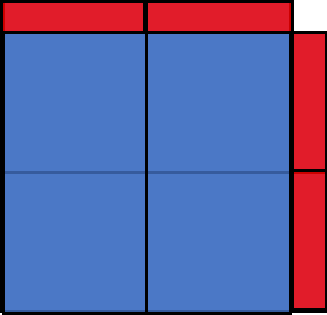
\includegraphics[width=0.4\textwidth]{crt-layout}
  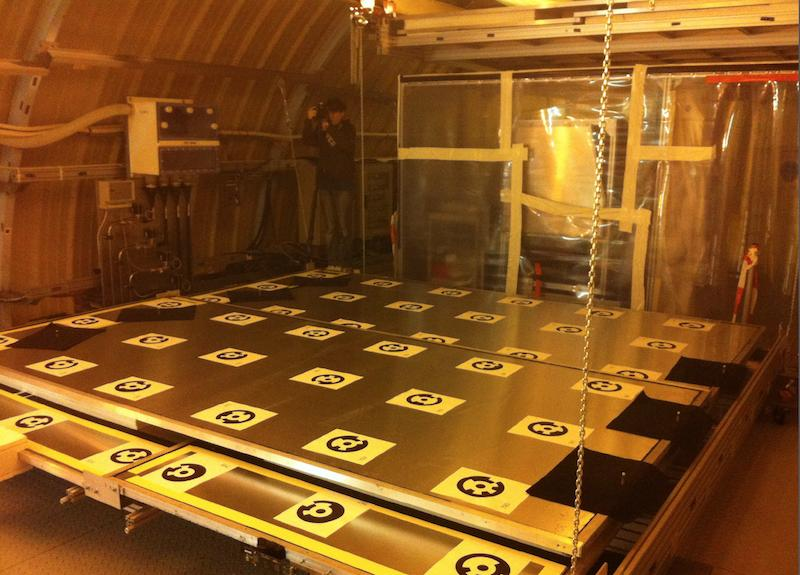
\includegraphics[width=0.5\textwidth]{double-chooz-layout}
\end{cdrfigure}

Possible locations for modules parallel to the upstream and downstream faces of the cryostat are under investigation. %Modules on these faces enable tagging and reconstruction of muons crossing the TPC volume. 
Full coverage of these faces, which would require eight four-module units, would allow field distortions to be mapped over the full TPC volume. 
\fixme{is this the plan?}
The CRT installation must preserve access to the outside of the cryostat, either by providing sufficient fixed space or through movement. 
\fixme{fixed space? let's clarify}
The modules must also avoid existing infrastructure. An appealing option for the upstream face is to make use of some of the existing APA rails. It is anticipated that a rails-and-hanger system identical to the APA design for both the upstream and downstream CRT modules will be used. Figure~\ref{fig:schematic-crt} shows a possible arrangement employing 24 modules (six four-module units). In this arrangement, data is taken with the downstream modules in two positions to cover the full TPC volume.
\fixme{two positions not clear}

\begin{cdrfigure}[Schematic view of upstream and downstream cosmic ray detectors]{schematic-crt}{Schematic view of upstream and downstream cosmic ray detectors}
 % \includegraphics[width=0.6\textwidth]{schematic-crt}
\end{cdrfigure}


%%%%%%%%%%%%%%%%%%%%%%%%%%
\subsection{Module position survey}

To allow a survey of module positions, each module includes four precision holes tied 
\fixme{holes aren't `tied' Are they lined up with the positions?}
directly to the scintillator strip positions. Double Chooz performed a photogrammetric survey using retroreflective balls installed in these holes along with a dozen coded optical targets attached to each module. This allowed them to determine module positions to $\pm$2\,mm. Figure~\ref{fig:dc-retroreflectiveballs} shows a sample photograph used for the survey. Figure~\ref{fig:dc-retroreflective-model} shows the model resulting from the combination of photographs.

\begin{cdrfigure}[Photo of Double Chooz far detector $y$-layer modules]{dc-retroreflectiveballs}{Photograph of Double Chooz far detector $y$-layer modules with retroreflective balls installed}
  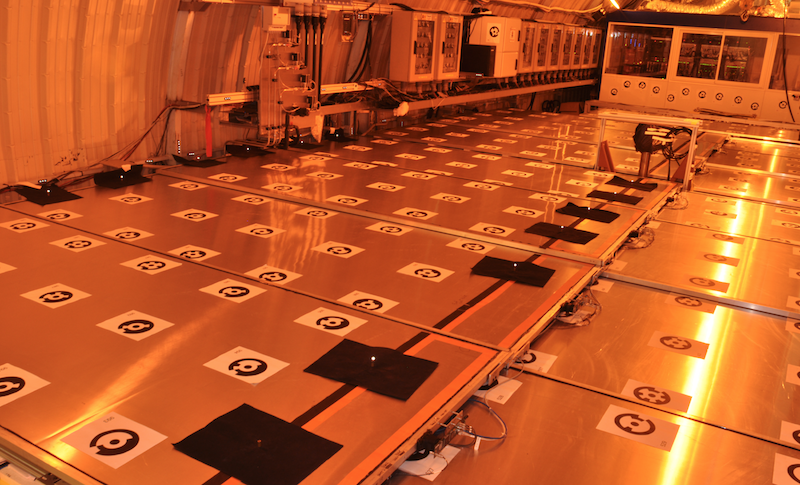
\includegraphics[width=0.7\textwidth]{dc-retroreflectiveballs}
\end{cdrfigure}


\begin{cdrfigure}[Model of Double Chooz $y$-layer modules]{dc-retroreflective-model}{Photomodeler model of Double Chooz $y$-layer modules showing retroreflective ball and coded target positions}
  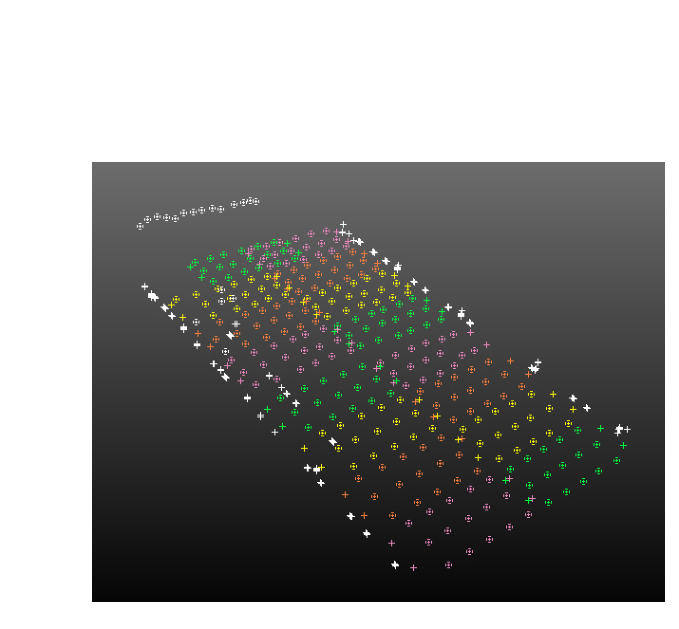
\includegraphics[width=0.8\textwidth]{dc-retroreflective-model}
\end{cdrfigure}


%%%%%%%%%%%%%%%%%%%%%%%%%%
\subsection{DAQ and readout}

The CRT uses its own readout. This readout produces a series of time ADC values and time stamps for hit strips, and makes use of a ProtoDUNE-SP global clock and sync pulse to enable merging with TPC information -- pseudo-online -- using time stamps. Note that the entire CRT system is isolated from the detector ground; it uses the building ground.

%%%%%%%%%%%%%%%%%%%%%%%%%%
\subsection{Testing of modules during installation}

All modules, PMTs, and front-end readout boards have been fully tested. Prior to installation, QA/QC procedures identical to those used for the Double Chooz installation will be used. Each module is first equipped with a reference PMT and front-end board. Using the same well-characterized PMT + readout board for all modules allows efficient checking for light leaks and other module defects. Once the light-tightness and proper function of the module is verified, the final PMT and PMT board are installed. The function of the PMT/PMT-board combination and the light-tightness of the PMT installation is checked before the module is put into position.
